\section{System Implementation}

\begin{figure*}[t]
 \begin{center}
  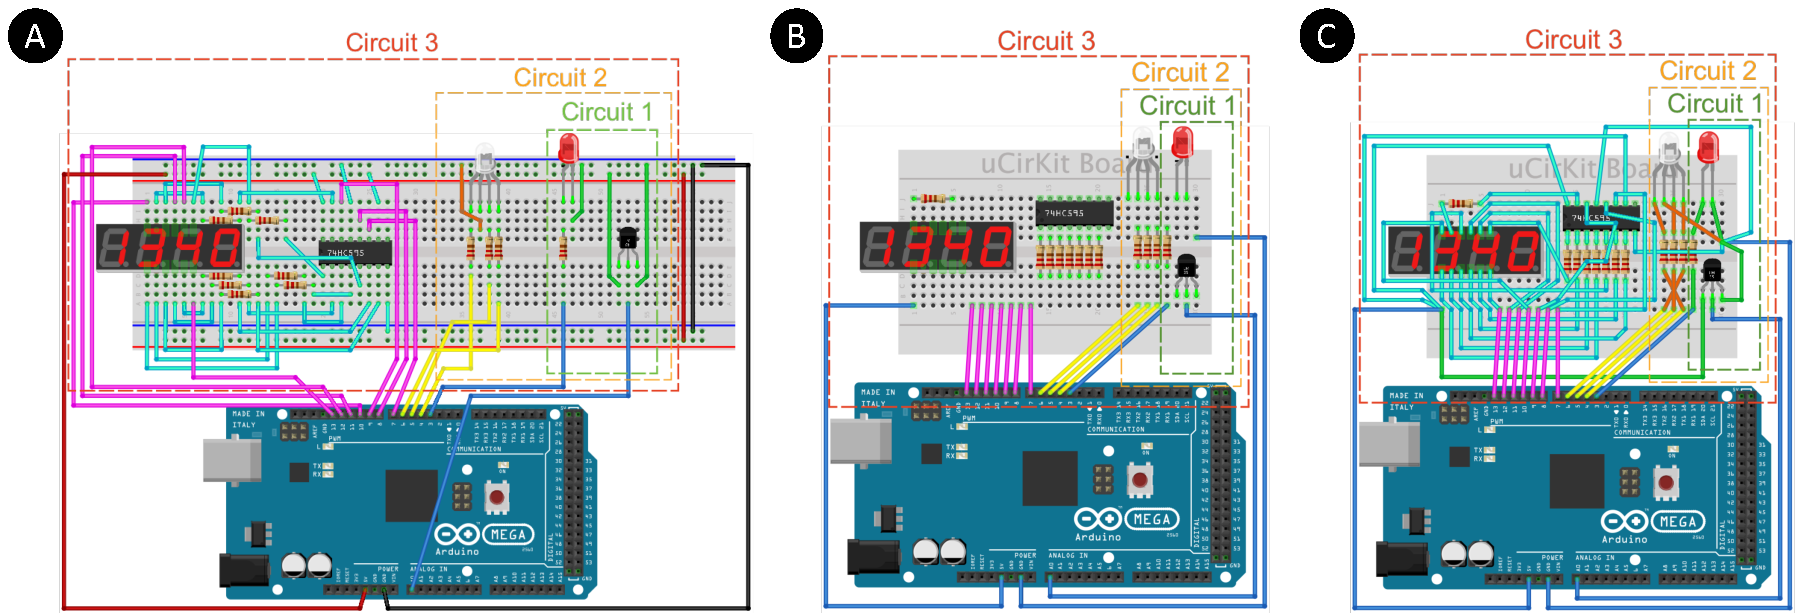
\includegraphics[width=2\columnwidth]{figures/Fritzing_Schematics_v3.pdf}
  \caption{
    Circuit 1 consists of a temperature sensor (LM35) and a LED that turns on as the temperature rises 3\textcelsius.
    Circuit 2 has a RGB LED which changes color smoothly from aqua to green to red every increment of 3\textcelsius.
    Circuit 3 is with a IC chip 74HC595 and a four-digit seven segment display  to show the temperature reading in Celsius.
    (A) and (B) are Fritzing schematics for breadboard and \papertitle, respectively. (C) shows connection arrangements hidden beneath \papertitle\ on a PCP.
  }
  \label{fig:Chosen_Circuits}
  \end{center}
\end{figure*}

% \begin{figure*}[t]
%  \begin{center}
%   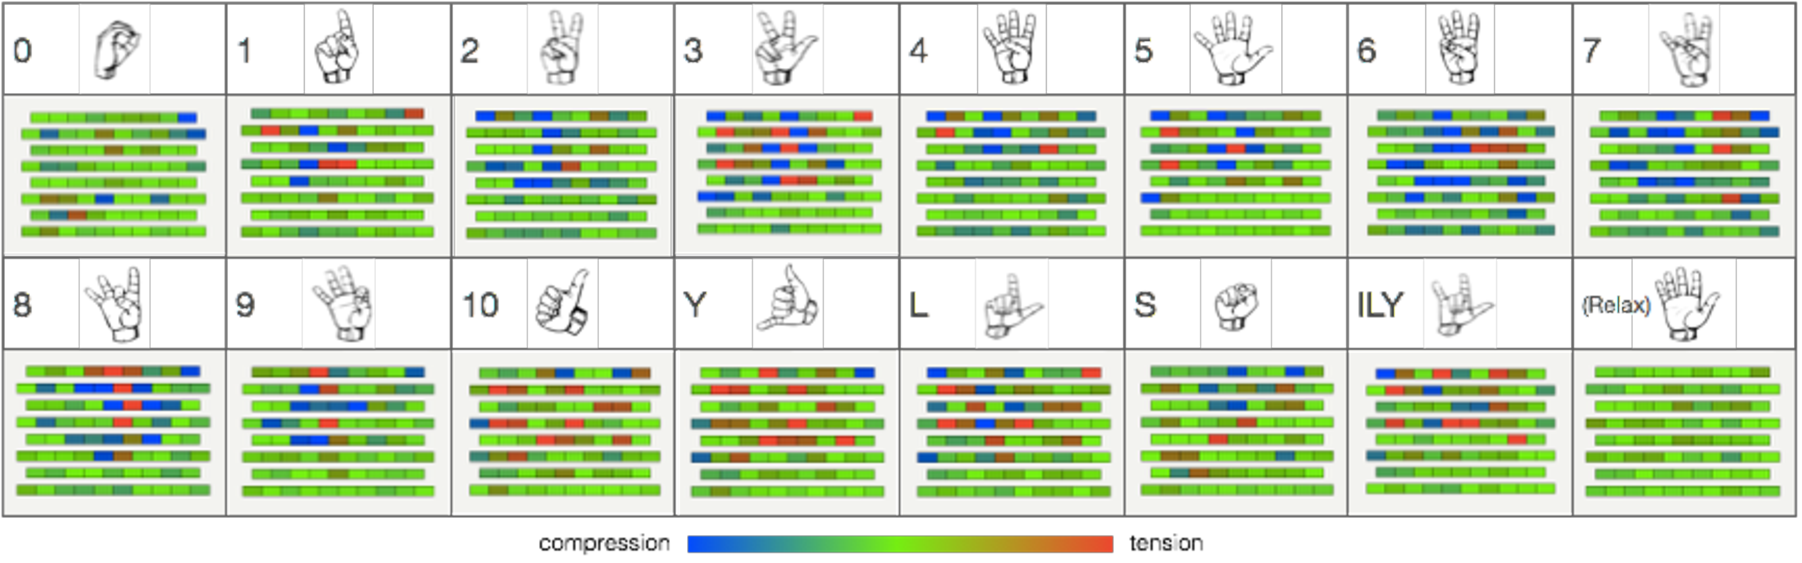
\includegraphics[width=2\columnwidth]{figures/user16GesturesSV_v3.pdf}
%   \caption{ 16 heat maps display all 16 gestures performed by one of the participants. Each entry is an average heat map of 10 trials of a gesture. The sensor reading patterns are significantly different across 16 gestures.
%   }
%   \label{fig:user16GesturesSV}
%   \end{center}
% \end{figure*}

Among the related works in the previous section, a breadboard provides easy modification by its pluggable mechanism, and PCP offers fast wiring by printing out conductive ink. Thus, we present a new rapid prototyping tool, \papertitle, simultaneously adopting a pluggable and PCP fast wiring mechanism.

\subsection{Hardware}

% Since \cite{Instant_Inkjet_Circuits} presented a successful approach to inkjet printing circuits, we adopted a similar setup with a Brother DCP-J105 printer, silver nanoparticle ink NBSIJ--MU01, resin coated paper, and transparent PET film from Mitsubishi Paper Mill.

Since \cite{Instant_Inkjet_Circuits} presented a successful approach to inkjet printing circuits, we adopted a similar setup with a Brother DCP-J105 printer and materials from Mitsubishi Paper Mill.

As illustrated in Figure X, \papertitle\ possesses a multi-layer design composed of customized PCBs. Figure X is the top layer consisting of 10-by-30 female headers resembling the appearance and the pluggable mechanism of a breadboard. Figure X indicates the bottom layers where pieces of PCP are placed. The wiring on each piece of PCP determines the connections for the component pins on the top layer. Despite showing only X layers in Figure X, \papertitle\ can stack up to even more layers to create more connections which support more complicated circuits.

Each pin and contact pad in zone A on both the top layer and the bottom layers connects to its corresponding pad on zone B. Each pad in zone B then contacts and electrically connects to its neighboring layers through a compressible on-board contact spring, part number OG-320816 (Figure X). Pads in zone A on the bottom layers are also equipped with the same contact spring to push against the conductive ink on a PCP to form reliable physical contacts. Lastly, the layers and pieces of PCP are assembled and stacked up through tightening four screws on 4 corners.

\subsection{Software}

To create wire routing on PCP for \papertitle, the Breadboard tab in Fritzing \cite{Fritzing} functions as an interface (Figure X) for users to place components and arrange connections on a custom part, \papertitle. Then, the connection information saved in a Fritzing file, extracted through a Python script, is exported to a PCB design software, EAGLE \cite{EAGLE} where final connection arrangements and autorouting for PCP are created via EAGLE user language programming (ULP) scripts.


% \begin{figure}
%   \begin{center}
%   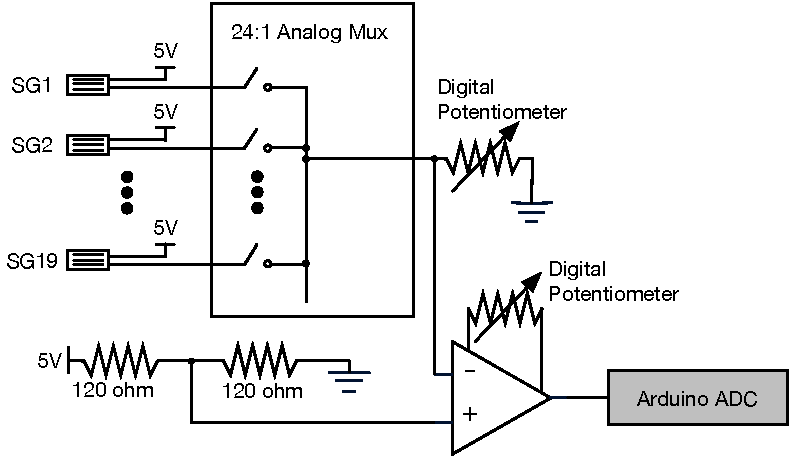
\includegraphics[width=1\columnwidth]{figures/Implementation.pdf}
%   \caption{The mechinical design of \papertitle }
%   \label{fig:FIGURE2}
%   \end{center}
% \end{figure}


% \begin{figure}
%   \begin{center}
%   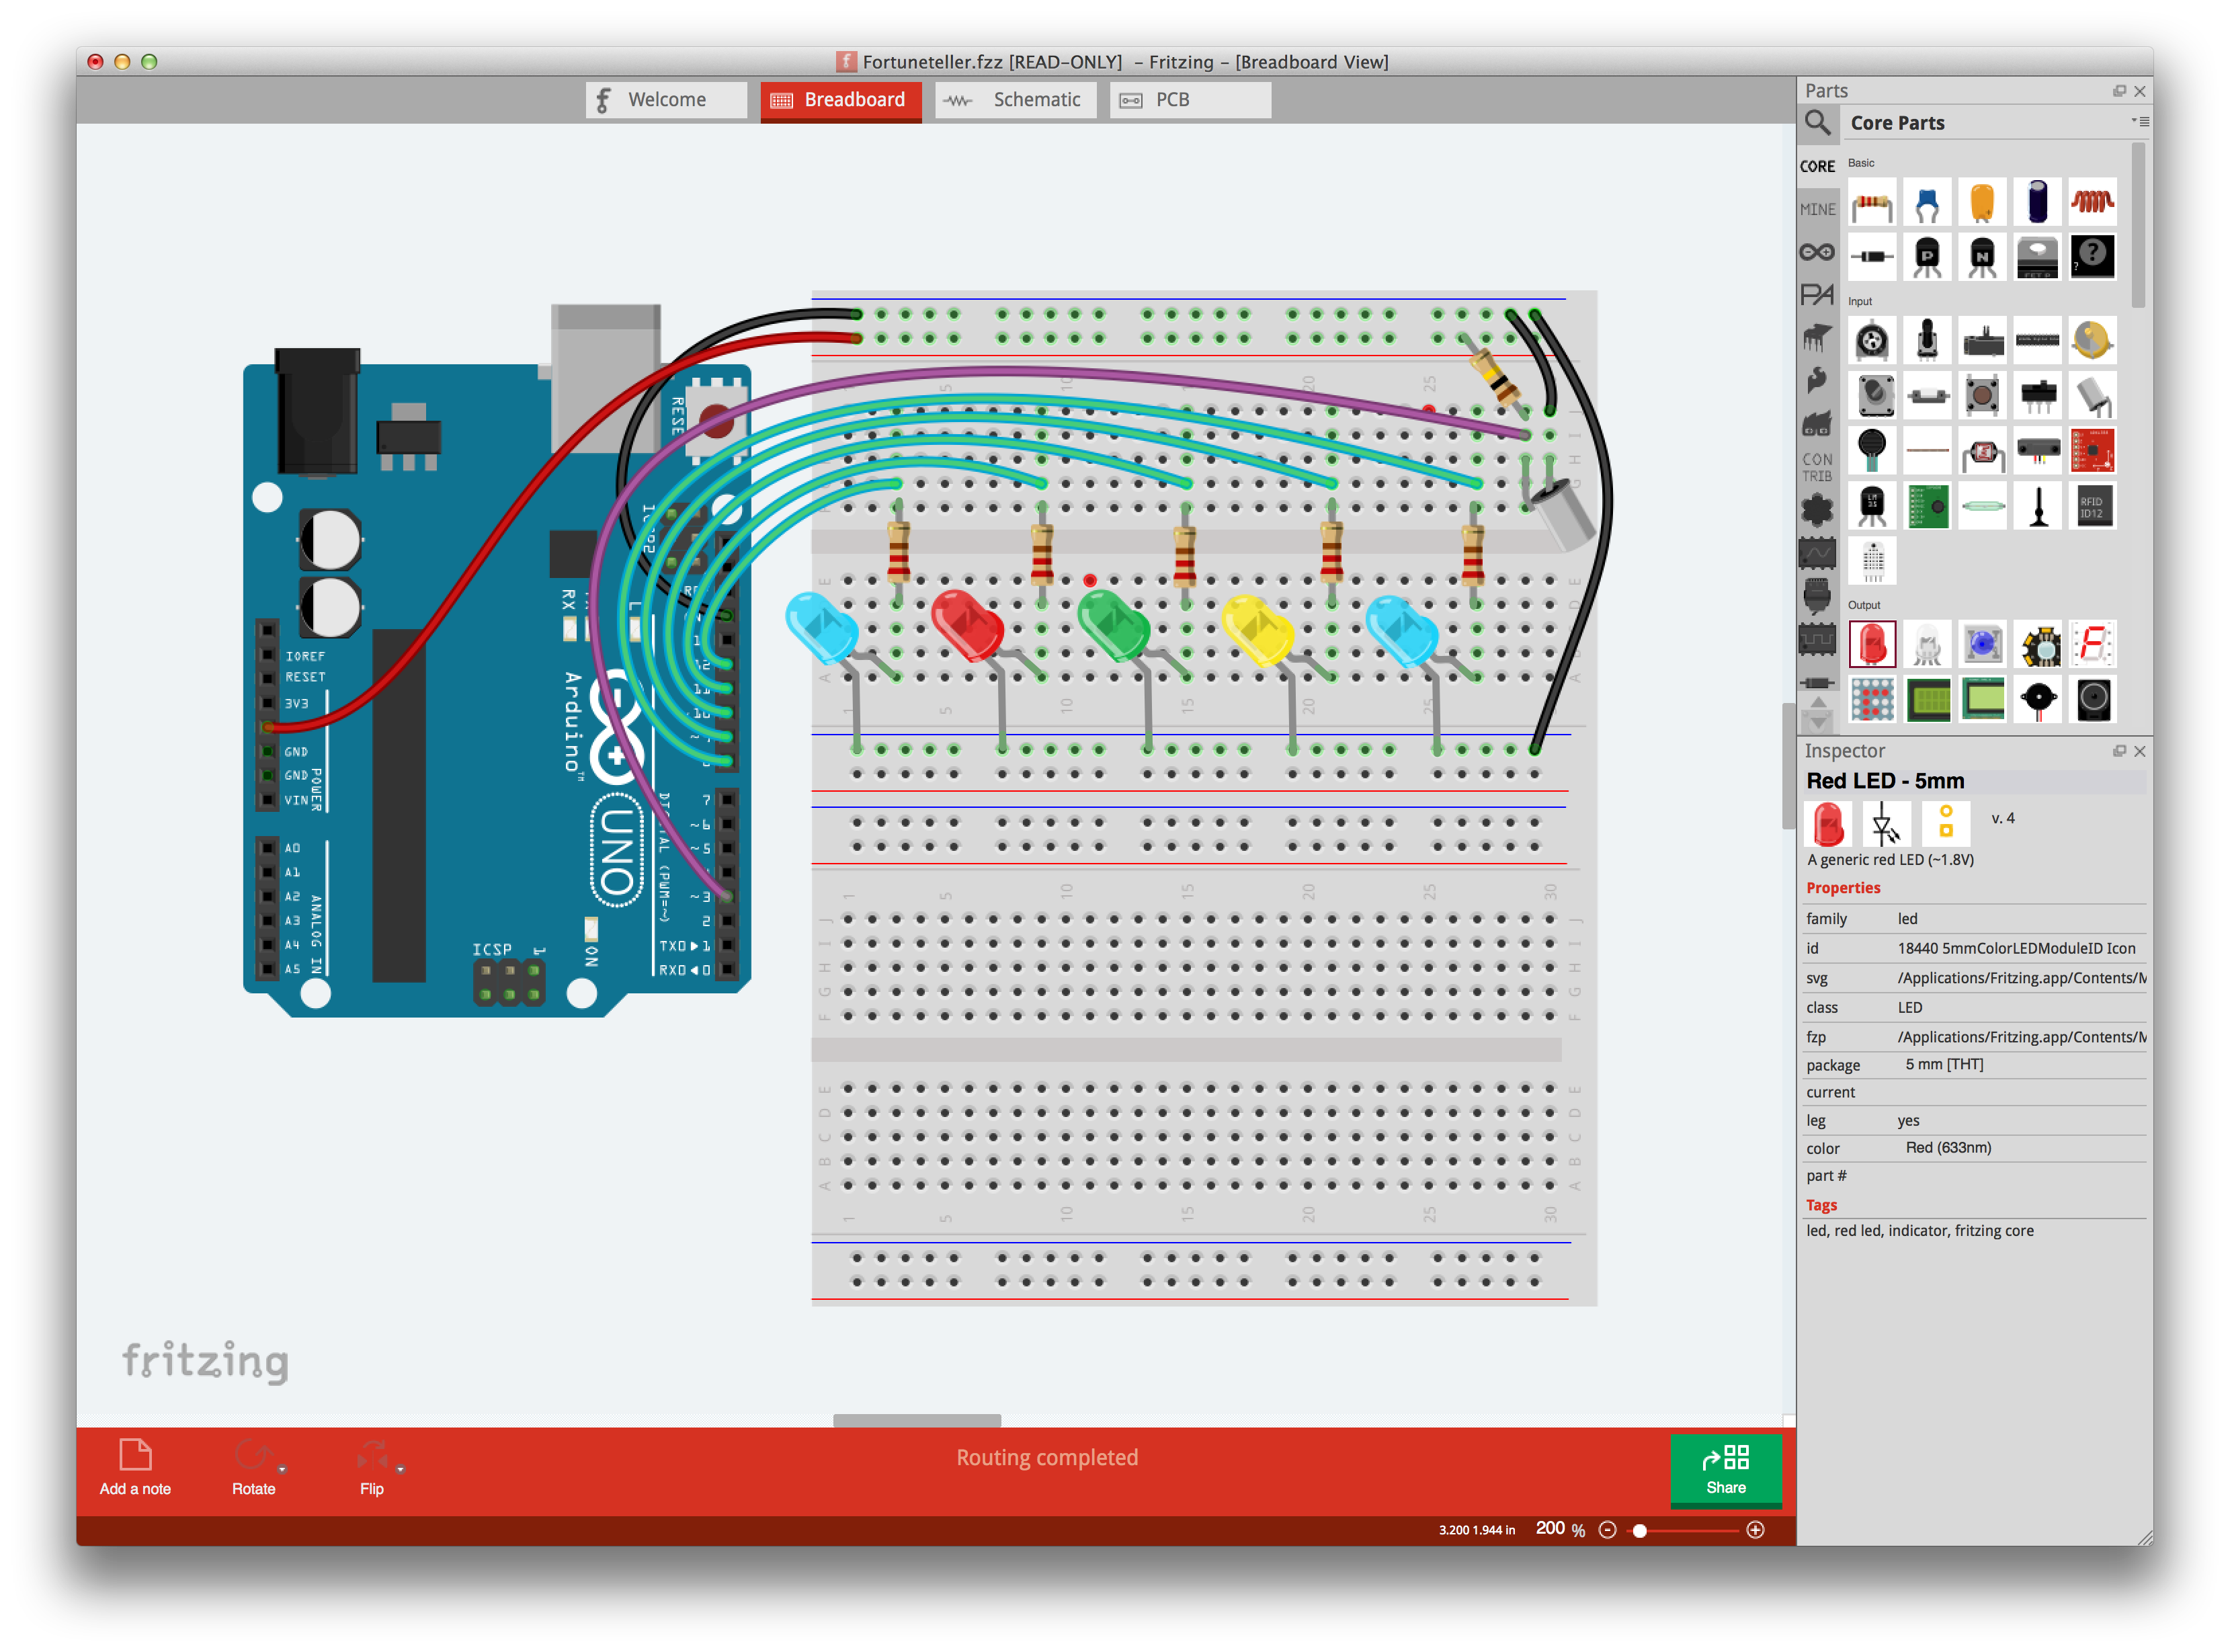
\includegraphics[width=1\columnwidth]{figures/GUI.png}
%   \caption{\papertitle also provides users a graphic user interface to help them design circuits efficiently.}
%   \label{fig:FIGURE4}
%   \end{center}
% \end{figure}